\section{Résultats et interprétations}

Nous avons fait tourner cette simulation pour une durée totale physique de 7284 secondes.

\subsection{Suivi de la courbe en S}
Les solutions pour chaque $r$ de la branche supérieure déterminées par dichotomie ne sont pas équivalentes aux branches atteintes dans la simulation. Nous pouvons voir sur la figure (\ref{fig:qmap}) en rouge la branche déterminée par dichotomie correspondant à $\tau_\mathrm{ff} = 0.06 $ et en blanc celle correspondant à la valeur théorique $\tau_\mathrm{ff} = 1$. Les possibles raisons de ces écarts sont dévelopés partie (\ref{sec::pistes}). La simulation est bien en accord avec le passage d'un disque optiquement épais à un disque optiquement mince. Nous pouvons voir figure (\ref{fig:c1.eps}) et (\ref{fig:c20.eps}) comment se comporte le système du point de vue de ces deux grandeurs physiques. 
 

\begin{figure}
  \begin{center}
    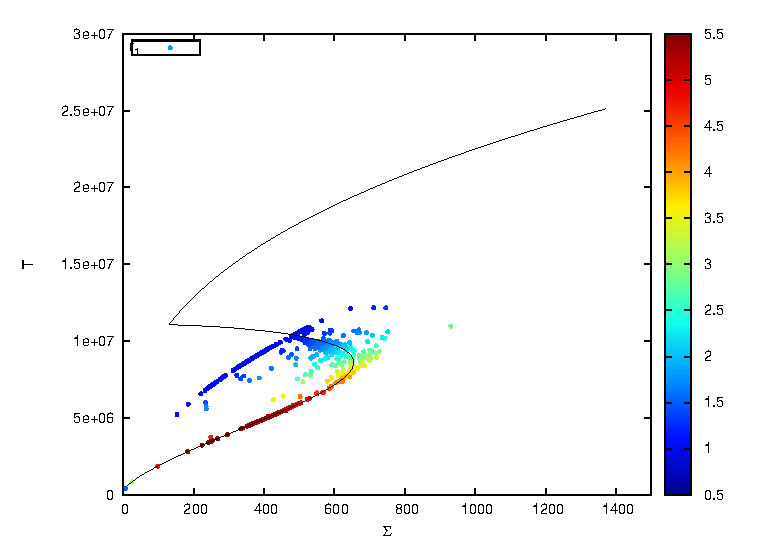
\includegraphics[]{c1.eps}
  \end{center}
  \caption{$T=f(\Sigma)$, $\Delta t = 7284 s$ (durée de la simulation) pour $r_{1}$. Le gradiant de couleur représente les valeurs de $\tau_\mathrm{ff}$}
  \label{fig:c1.eps}
\end{figure} 

\begin{figure}
  \begin{center}
    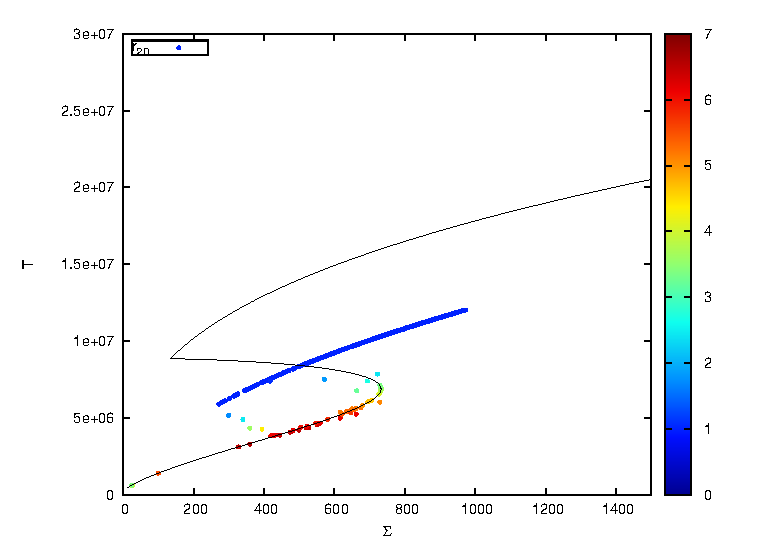
\includegraphics[]{c20.eps}
  \end{center}
  \caption{$T=f(\Sigma)$, $\Delta t = 7284 s$ (durée de la simulation) pour $r_{20}$. Le gradiant de couleur représente les valeurs de $\tau_\mathrm{ff}$}
  \label{fig:c20.eps}
\end{figure}

\subsection{Évolution de la luminosité}

Pour des valeurs de $\dot{M}_0$ suffisamment faible, le disque converge comme prévu vers la solution stationnaire. Ce régime est atteint en un temps d'environ 3000s. C'est un régime qui correspond à un transfert total de matière de l'extérieur du disque jusqu'à tomber dans le trou noir. On s'attend à avoir une luminosité constante qui traduit la conversion partielle de l'énergie potentielle de gravité en énergie thermique, et ainsi en énergie radiative via le terme $L_\mathrm{tot} = \int_{r_\mathrm{min}}^{r_\mathrm{max}} 2\pi r Fz\ \mathrm{d}r$. Le tracé de la luminosité est donné en figure \ref{eq:Lstable} et est en accord avec le comportement physique attendu. Dans un diagramme $\Sigma-T$, cela correspond à un point fixe et stable de la courbe en S.

\begin{figure}
  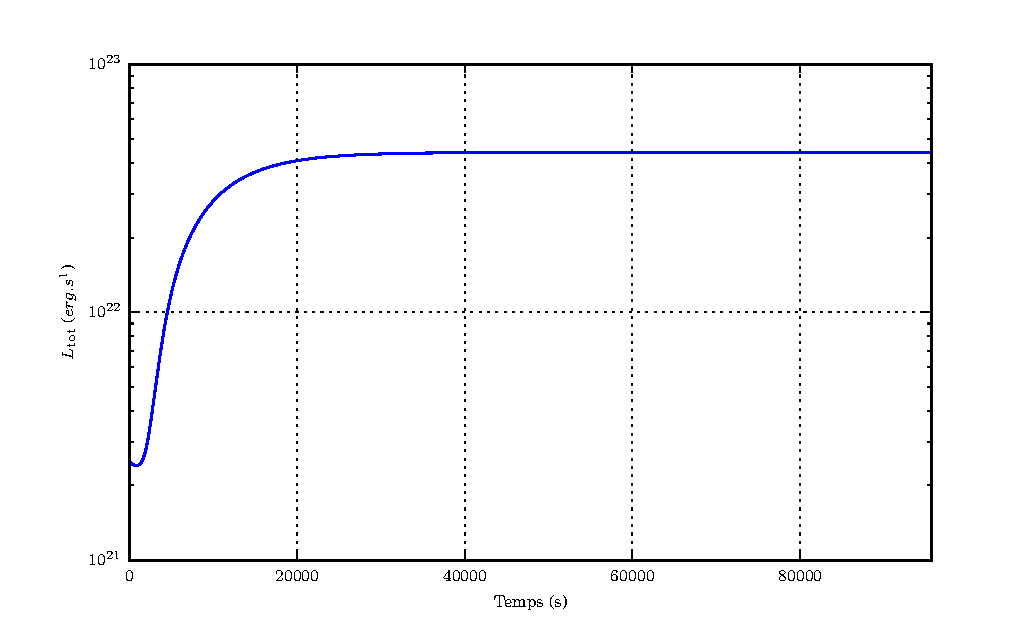
\includegraphics{figures/Ltot_fonction_t_stable.pdf}
  \caption{Évolution de la luminosité totale du disque $L_\mathrm{tot}$ en fonction du temps pour un taux d'accrétion faible $\dot{M}_0 = 10^{-4}\dot{M}_c$. Le disque atteint rapidement son état stationnaire où la luminosité est constante et vaut ici $4.4\ 10^{22}\mathrm{erg.s^{-1}}$}
  \label{eq:Lstable}
\end{figure}

Lorsqu'on perturbe le disque en augmentant le taux d'accrétion, on doit finir par atteindre un régime instable. C'est ce qu'on observe lorsqu'on augmente $\dot{M}_0$ dès qu'un équilibre est atteint. La simulation montre que la luminosité totale du disque n'est pas constante et possède des sursauts, correspondant à l'instabilité, représenté sur la figure \ref{fig:Ltot_function_t}. Cette figure présente des incurvations de la luminosité qui correspondent à l'augmentation de $\dot{M}_0$ au bord extérieure. L'instabilité se déclenche plus rapidement que l'arrivée au point stable de la figure \ref{fig:Lstable} car le critère de stabilité déclanchant l'augmentation du taux d'accrétion n'attend pas l'équilibre en $L_\mathrm{tot}$.

Dans un premier temps, qui correspond à l'ajout de plus en plus important de matière ($\dot{M}_0$ croissant), sa luminosité augmente lentement dans le domaine énergétique de $10^{21}$ à $10^{24}\ \mathrm{erg.s^{1}}$. Lorsque le disque entre dans l'instabilité, la luminosité croît fortement pour atteindre $10^{25}$ à $10^{27}\ \mathrm{erg.s^{-1}}$. Un détail de la luminosité sur une instabilité est donné sur la figure \ref{fig:Ltot_instabilite}. La non-régularité de la luminosité (sa déviation standard est de l'ordre de grandeur de sa moyenne) laissent à penser que la simulation numérique ne résoud pas correctement l'instabilité. En revanche, on constate que la luminosité moyenne durant l'instabilité est $7.6\ 10^{25}\mathrm{erg.s^{-1}}$, valeur qui est un ordre de grandeur plus important que la luminosité dans le régime stable.
\begin{figure}
  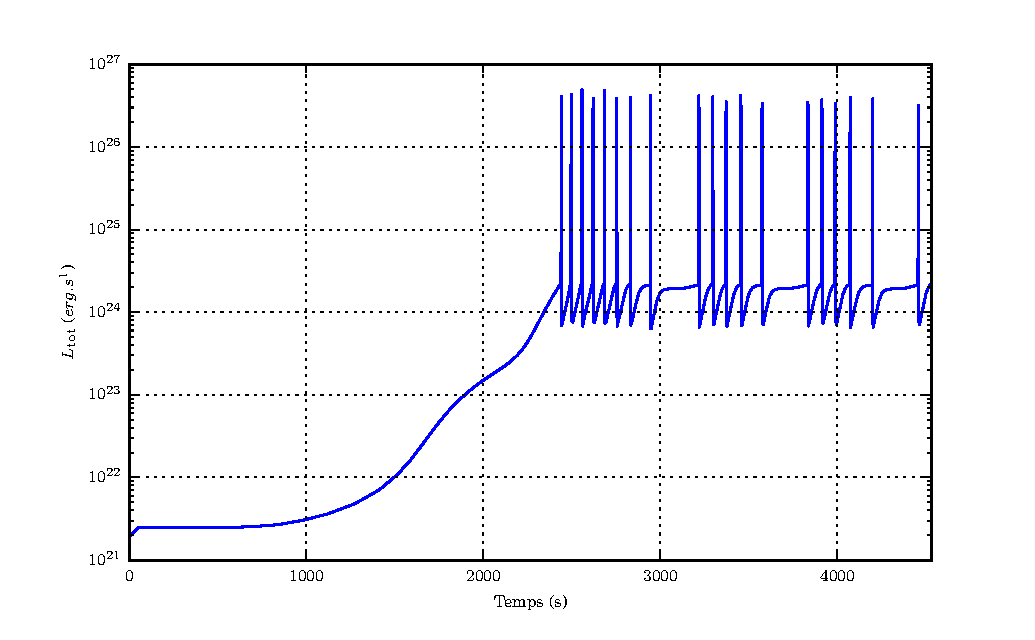
\includegraphics{figures/Ltot_fonction_t.pdf}
  \caption{Simulation de la luminosité $L_\mathrm{tot}$ au cours du temps, en partant avec $\dot{M}_0 = 10^{-4}\dot{M}_c$. Dès qu'un équilibre est atteint, $\dot{M}_0$ est augmenté. Cela se traduit par des incurvations successives de la luminosité. L'instabilité se déclenche à $t \approx 2300s$ et se répète régulièrement.}
  \label{fig:Ltot_function_t}
\end{figure}

\begin{figure}
  
  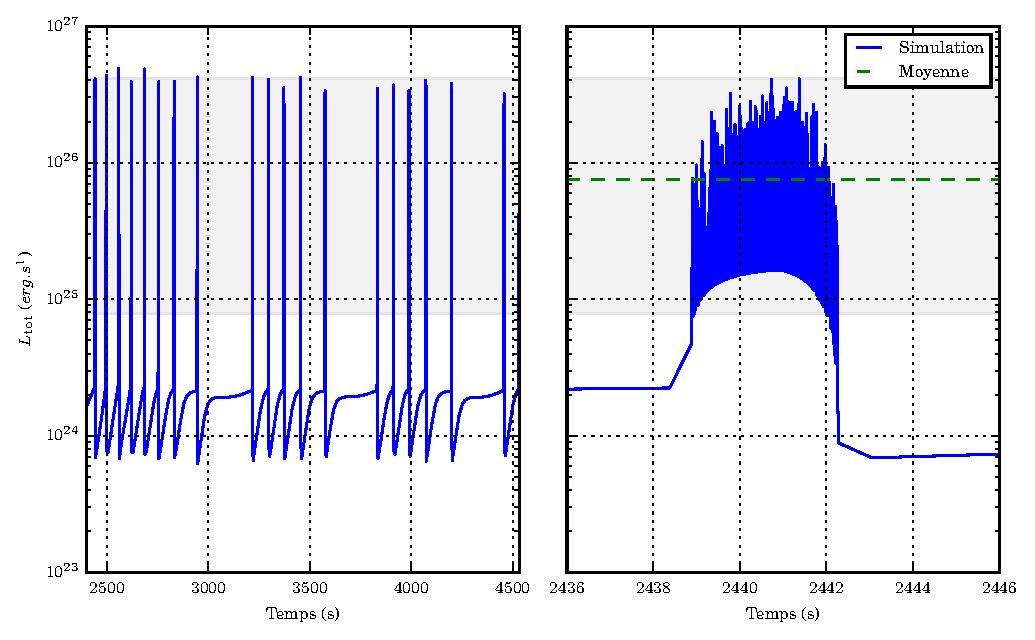
\includegraphics{figures/Ltot_fonction_t_doublecheeseburger.pdf}
  \caption{Simulation de la luminosité $L_\mathrm{tot}$ lors de l'instabilité. À gauche, un dizaine d'instabilités sont observées. À droite, un zoom sur la première instabilité. Sa moyenne est tracée en verte. L'applat gris est délimité par le maximum et le minimum de luminosité sur l'instabilité. On notera par ailleurs que la déviation standard de la luminosité y est du même ordre de grandeur que sa moyenne.}
  \label{fig:Ltot_instabilite}
\end{figure}
%%% Local Variables:
%%% mode: latex
%%% TeX-master: "rapport"
%%% End:
